\chapter{Motivation}


%===================================================================================================%
\section{Introduction}
%===================================================================================================%



%===================================================================================================%
\section{What the fuck is Serverless?}
%===================================================================================================%

"Serverless" is \textbf{the} new hype technology prominently featured in more than five Gartner Hype-Cycle reports that identify trends and emerging technologies that will shape the industries future. 
\autocite{Smith2017Hype2017}
\autocite{Weiss2017Hype2017}
\autocite{Natis2017Hype2017}
\autocite{Walker2017Hype2017}
\autocite{DawsonPhilip2017Hype2017}
But what is "serverless"? Many attempted to define the term but Mike Roberts formulated the most universal description:  

\blockquote{\guillemotleft \ ["Serverless" refers to] custom code that's run in ephemeral containers (Function as a Service or "FaaS").[...] Such architectures remove the need for the traditional 'always on' server system sitting behind an application. Depending on the circumstances, such systems can significantly reduce operational cost and complexity. \guillemotright\autocite{Roberts2016ServerlessArchitectures}}

To understand this very broad but commonly accepted definition of "serverless", the first prerequisite is to understand what a server is and how a serverless system differs from it. \textquote{A server is a computer designed to process requests and deliver data to another computer over the internet or a local network}\autocite{TheServer}, meaning that a server poses as an accessible endpoint that waits for requests from clients and responds to them. It is \textit{continuously} running, even if there is no task to be done in order to be ready for incoming requests. This waiting-time is called "idle time" presents the most significant difference between servers and serverless systems: while the server \textbf{waits} for incoming requests to process them, in a serverless context, a computational unit is created for every incoming request.

\begin{figure}[ht]
    \includegraphics[width=0.9\linewidth]{images/drawio/3tier-oneclient.png}\centering
    \caption {Classic Three-Tier Architecture}
    \label{fig:3tier1client}
\end{figure}

Take the case of an online-shop. Its extremely simplified architecture diagram of it can be seen in Figure \ref{fig:3tier1client}. It depicts the classic three-tier-model that consists of the presentation (client), logic (server) and data (database) tier.\autocite{Ramirez2000Three-TierArchitecture} Let's assume the customer wants to $buy$ one item. First, the client sends a request to the shop's server, which will process it by querying the database if enough items are in stock, performing the purchase (writing to the database) and lastly responding to the client whether his request was successful or not. In other words, the action of buying one item is realized as a sequence of a finite amount of steps that have to be passed in order to achieve the desired result. These steps are the the same every time a client issues the $buy$ request. But what happens if multiple customers want to $buy$ an item simultaneously? \\
% As illustrated in Figure \ref{fig:3tierNclient}, the amount of steps that have to be performed concurrently to process every request in a timely manner grows with every added client. \\
% \begin{figure}[ht]
%     \includegraphics[width=0.9\linewidth]{images/drawio/3tier-multipleclient.png}\centering
%     \caption {Classic Three-Tier Architecture with multiple Clients}
%     \label{fig:3tierNclient}
% \end{figure}
The amount of steps that have to be performed concurrently to process every request in a timely manner grows with every added client but since a server operates on a finite amount of resources, eventually a performance-wise degradation of service occurs. Traditionally, more servers and therefore more available compute power would be added to the system to cope with this challenge. Unfortunately, this approach results in a very inelastic provision of resources which is illustrated in Figure \ref{graph:provisionedComputePowerServer}. To further simplify, let's assume that every server can handle exactly 1000 clients. If 1001 clients simultaneously connect to the system, at least two servers have to be running to satisfy the calls. 

\begin{figure}[ht]
    \begin{tikzpicture}
        \begin{axis}[
                ,xlabel         = $\# Requests$
                ,ylabel         = {$Provisioned \, Compute \, Power$}
                ,yticklabels    = {,,}
                ,xticklabels    = {,,}
                ,axis x line    = bottom
                ,axis y line    = left
                ,domain         = 0:6
                ,ymajorgrids    = true
                ,grid style     = dashed
                ]
            \addplot [const plot, no marks, color=blue] coordinates {(0,1) (1,2) (2,3) (3,4) (4,5) (5,6)};
            \addplot [color=white]{x};
        \end{axis}
    \end{tikzpicture}\centering
    \caption {Provisioned Compute Power: Server Model}
    \label{graph:provisionedComputePowerServer}
\end{figure}

\begin{figure}[ht]
    \includegraphics[width=\linewidth]{images/drawio/lambda.png}\centering
    \caption {Serverless Architecture (simplified)}
    \label{fig:serverlessArchHighlevel}
\end{figure}


As depicted in Figure \ref{fig:serverlessArchHighlevel} \textcolor{red}{TODO: Dienstag}
\ref{graph:provisionedComputePowerServer} shows how this bottleneck scales

\begin{figure}[ht]
    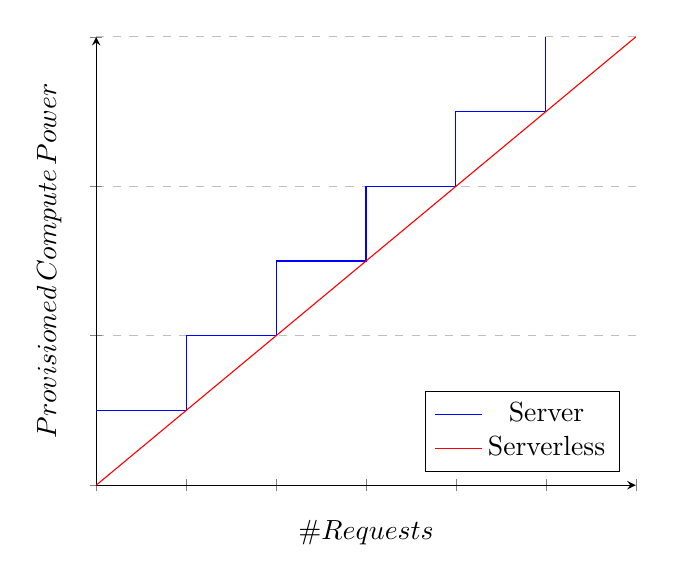
\begin{tikzpicture}
        \begin{axis}[
                ,xlabel         = $\# Requests$
                ,ylabel         = {$Provisioned \, Compute \, Power$}
                ,yticklabels    = {,,}
                ,xticklabels    = {,,}
                ,axis x line    = bottom
                ,axis y line    = left
                ,domain         = 0:6
                ,legend pos     = south east
                ,ymajorgrids    = true
                ,grid style     = dashed
                ]
            \addplot [const plot, no marks, color=blue] coordinates {(0,1) (1,2) (2,3) (3,4) (4,5) (5,6)};
            \addlegendentry{Server}
            \addplot [color=red]{x};
            \addlegendentry{Serverless}
        \end{axis}
    \end{tikzpicture}\centering
    \caption {Provisioned Compute Power Comparison: Server/Serverless}
    \label{graph:provisionedComputePowerComparison}
\end{figure}



%===================================================================================================%
\section{Why Serverless?}
%===================================================================================================%


was ist serverless? was ist der unterschied zwischen serverless und server

The \acf{IoT} is one of the major growth markets of the recent years and is expected to reach a global revenue of \$457B by the end of 2020, attaining a \acf{CAGR} of 28.5\% over four years.\autocite{Columbus20172017Forecasts} Looking at the most common usecases for IoT applications, it is clear that the prevailing real-life scenarios can be characterized by ubiquitous sensors numbering in the millions or even billions constantly monitoring physical objects, events and humans alike. Right now, these observations are often communicated to a cloud data center for various analyses that in turn trigger reactions to the observed events which aims to improve the efficiency and reliability of systems and generate valuable insights.\autocite{Yannuzzi2014KeyComputing} \\
This pattern results in a closed-loop \acf{OODA} cycle, where the the three major components are the information \textit{producers} (sensors), the \textit{cloud endpoint} and the \textit{consumer} or \textit{processor}.\autocite{Shukla2017BenchmarkingApplications} Especially this closed-loop characteristic of IoT applications is essential for their effective use and a low latency between observing events and processing them is therefore a fundamental requirement. To derive actionable insights that have a business impact, it is essential to process the data ingress in near real-time since information often have a time-to-live are only valid for a short amount of time, hence a rapidly scaling processor-concept that is performant enough to digest the data ingress is an imperative system component. \acf{ESP} approaches are an obvious solution to this challenge and reference IoT solutions from cloud providers \footnote{\url{https://aws.amazon.com/iot-core/features/}}\textsuperscript{,}\footnote{\url{https://microsoft.com/en-in/cloud-platform}} include some sort of event streaming.


%===================================================================================================%
\section{Scientific Body of Knowledge}
%===================================================================================================% 



%===================================================================================================%
\section{Research Gap/Question}
%===================================================================================================%


The purpose of this research is to evaluate the suitability and viability of the serverless architecture pattern by comparing them in a prototypical scenario. The result will be a simplified decision-framework for architects that enables them to decide if a "serverless" architectural approach is fitted for their stream-processing use-case.

One sub-objective is to asses the current industry understanding of "serverless" and evaluate the suitability and viability of this architecture pattern.
Moreover, it is supposed to assist the process of highlevel system design by providing a reference and guidance by introducing fPaaS\footnote{"Function-Platform-as-a-Service". Defined by Gartner \autocite{Chandrasekaran2017EvolutionWhen}} capabilities and caveats.

%===================================================================================================%
\section{Summary}
%===================================================================================================%